% Gemini theme
% https://github.com/anishathalye/gemini

\documentclass[final]{beamer}

% ====================
% Packages
% ====================

\usepackage[T1]{fontenc}
\usepackage{caption}
\usepackage{subcaption}
\usepackage[superscript,biblabel]{cite}
\usepackage{lmodern}
\usepackage[scale=1.15,size=a0,orientation=portrait]{beamerposter}
%\usepackage[size=custom,width=90,height=130,scale=1.25]{beamerposter}
\usetheme{gemini}
\usecolortheme{labsix}
\usepackage{graphicx}
\usepackage{svg}
\svgsetup{inkscapeexe=/Applications/Inkscape.app/Contents/MacOS/inkscape}
\DeclareGraphicsRule{.ai}{pdf}{.ai}{}
\usepackage{booktabs}
\usepackage[none]{hyphenat}
\usepackage{amsmath}
\usepackage{amssymb}
\usepackage{tikz}
\usetikzlibrary{fit,backgrounds}
\usepackage{pgfplots}
\usepgfplotslibrary{fillbetween}


% ====================
% Lengths
% ====================

% If you have N columns, choose \sepwidth and \colwidth such that
% (N+1)*\sepwidth + N*\colwidth = \paperwidth
\newlength{\sepwidth}
\newlength{\colwidth}
\setlength{\sepwidth}{0.025\paperwidth}
\setlength{\colwidth}{0.3\paperwidth}

\newcommand{\separatorcolumn}{\begin{column}{\sepwidth}\end{column}}

% ====================
% Title
% ====================

\title{Mesoscopic thermodynamics of single-particle enzymatic reactions}

% REMOVED \inst{1}
\author{Filipe P. de Farias\inst{1} \and Francesco Corona\inst{2}  \and Michela Mulas\inst{1}}

\institute[UFC]{\inst{1}Post-graduate Programme in Teleinformatics Engineering, Federal University of Ceará, Brazil\\ \inst{2}School of Chemical Engineering, Aalto University, Finland}

% ====================
% Footer (optional)
% ====================
 %% REMOVED {  %\href{https://www.example.com}{https://www.example.com} 
  %\href{mailto:alyssa.p.hacker@example.com}{alyssa.p.hacker@example.com} }
\footercontent{
  \hfill
  Challenges in the Physics of Active and Biological Matter 2023
  \hfill
}
% (can be left out to remove footer)

% ====================
% Logo (optional)
% ====================

% use this to include logos on the left and/or right side of the header:
\logoright{\includegraphics[height=10cm,
%page=2,trim={17cm 21cm 3cm 5cm},clip
]{"graphics/brasao2_vertical_monocromatico"}}
\logoleft{\includegraphics[height=10cm,trim={50 50 50 50},clip]{"graphics/logo-31148-1"}}

% ====================
% Body
% ====================

\begin{document}

\setlength{\abovedisplayskip}{40pt}
\setlength{\belowdisplayskip}{40pt}

\begin{frame}[t]
\begin{columns}[t]
\separatorcolumn

\begin{column}{\colwidth}

%\begin{block}{Introduction}
%The energy transfer of systems at mesoscopic scale with stochastic dynamics which are open and out-of-equilibrium are the subject of study Stochastic Thermodynamics\cite{peliti2021stochastic,Falasco:2023aa}. 
%%
%\begin{itemize}
%\item Systems at equilibrium have {\bf reversible trajectory}, i.e. a transition of the system from the state $x \rightarrow x^\prime$ at a rate $k_{xx^\prime}$, its reversed transition $x^\prime \rightarrow x$ has the rate $k_{x^\prime x}=k_{xx^\prime}$.
%
%\item At {\bf non-equilibrium} a system is kept stationary by dissipating energy (local detailed balance) proportional to $\ln (k_{xx^\prime} / k_{x^\prime x})$\cite{10.21468/SciPostPhysLectNotes.32}.
%\end{itemize}
%{\bf Stochastic thermodynamics} (ST) deals with the interaction of mesoscopic, nonequilibrium physical systems with heat reservoirs in equilibrium.\cite{peliti2021stochastic} Such interactions are assumed to be the source of the randomness in the dynamics of the system, assigning to it a probability $p_x(t)$ of being in the state $x$ at time $t$.
%\begin{itemize}
%\item We will use the Michaelis-Menten kinetics as case of study for the ST.
%\end{itemize}
%\end{block}

\begin{block}{Michaelis-Menten theory}
The Michaelis-Menten kinetics models the kinetics of enzyme $E$ reacting with substrate $S$ forming complex $ES$ which releases product $P$ and enzyme according to the following chemical reaction network: 
\begin{equation*}
E + S \underset{k_{-1}}{\stackrel{k_1}{\rightleftharpoons}} ES \underset{k_{-2}}{\stackrel{k_2}{\rightleftharpoons}} E + P.
\end{equation*}
%
In this analysis, it is assumed that:
\begin{itemize}
\justifying
\item The amounts of $S$ and $P$ are considered to be much larger than of $E$ and $ES$ such that a reaction does not change considerably the quantities of $S$ and $P$;
\item The reactions are modeled as random interactions of the enzyme with the reservoir in equilibrium at temperature T formed by the solution of $S$ and $P$\cite{Seifert:2010aa}.
\end{itemize}
%
\begin{figure}
\centering
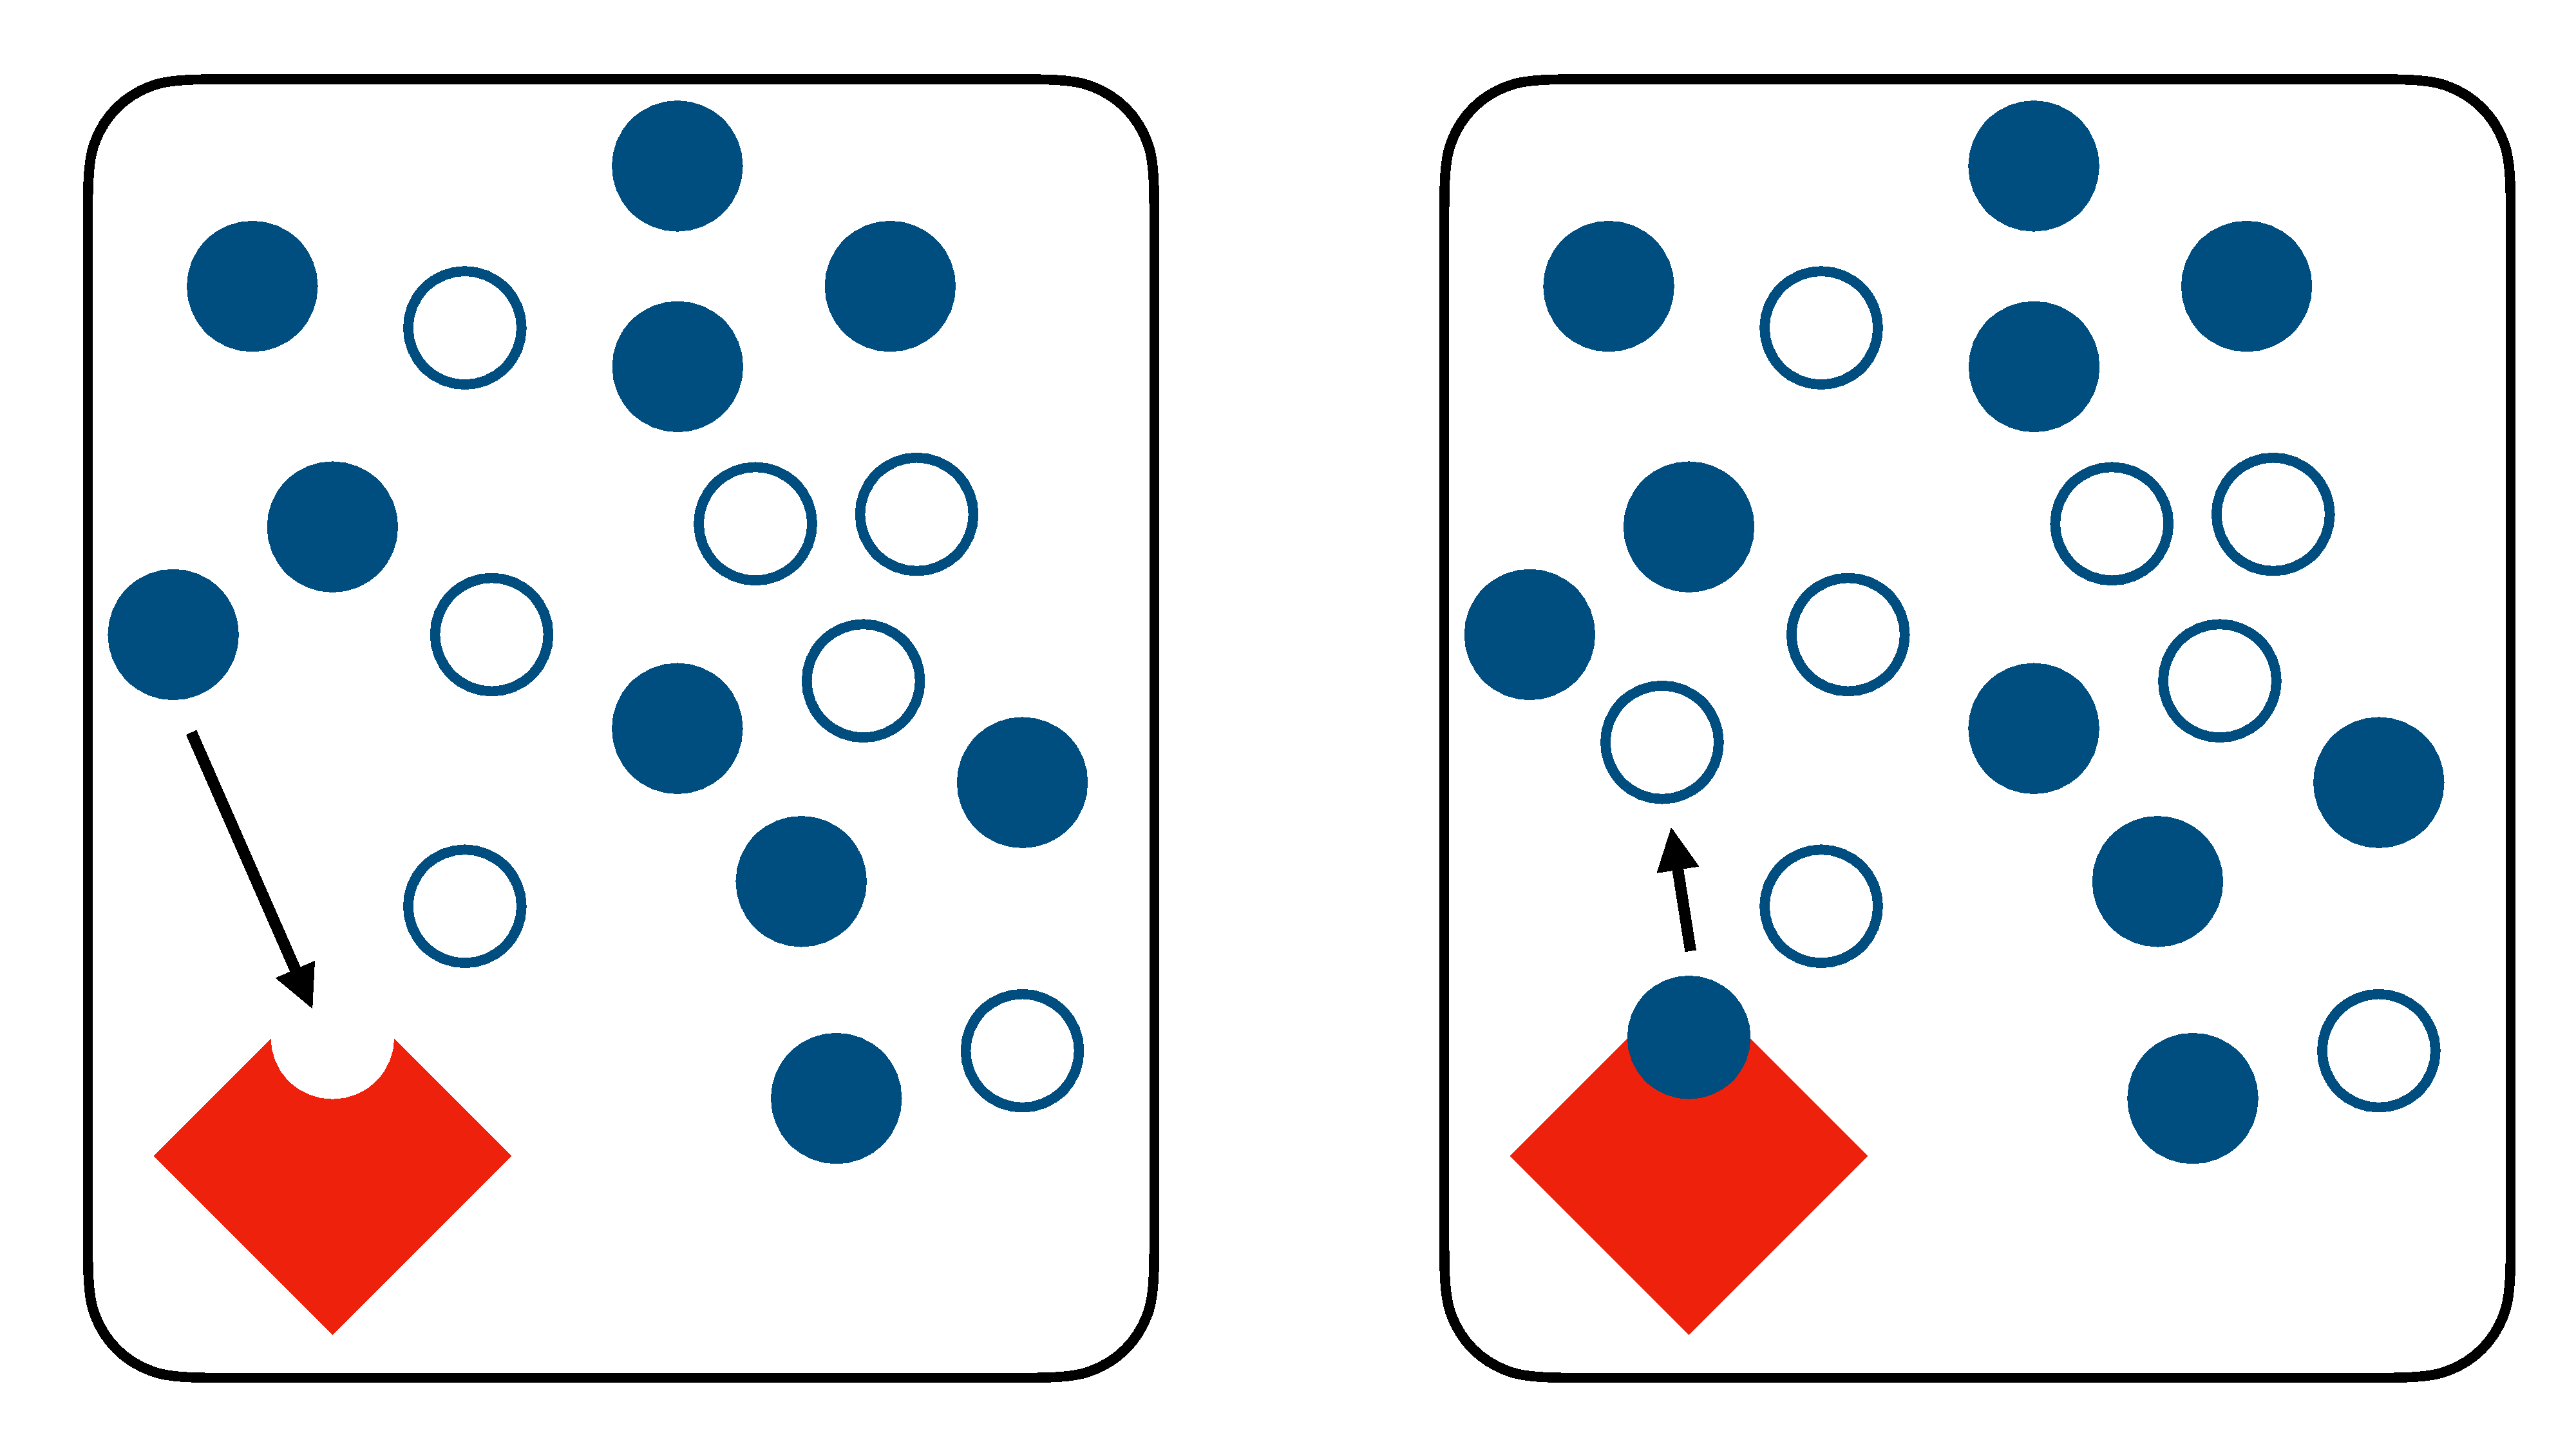
\includegraphics[width=.8\textwidth]{graphics/MichaelisMenten.pdf}
\caption{\justifying Figure adapted from Seifert (2010)\cite{Seifert:2010aa}, where the solution is composed by substrate (filled circle), product (empty circle) and single enzyme (red square). The single enzyme is interacting with the solution changing its state.}
\vskip-20pt
\end{figure}
%
The system considered consists of $n_E$ molecules of $E$ and $n_{ES}$ molecules of $ES$, being the system states $x \in \mathcal{X} : \{0,...,n_E\}\times \{0,...,n_E\}$.
%%
%\begin{itemize}
%\item Setting $n_E=n_{ES} = 1$ gives a system with one enzyme.
%\end{itemize}

%Considering only one enzyme, the states in which it is found is $E$ or $ES$, thus the number of molecules of each of them are $n_E \in \{0,1\}$ and $n_{ES} \in \{0,1\}$, respectively.
\begin{itemize}
\justifying
%%
%\item The states  of the system are $x \in n_E \times n_{ES}$
%
%\item The substrate $S$ and the product $P$ are {\bf chemostated}.
%\begin{figure}
%\begin{subfigure}[b]{0.45\textwidth}
%\centering
%\includesvg{graphics/2-state-graph.svg}
%\caption{}
%\label{fig 2-state-system}
%\end{subfigure}
%\begin{subfigure}[b]{0.45\textwidth}
%\centering
%\includesvg[scale=1.1]{graphics/ST-MM-prob.svg}
%\caption{}
%\label{fig 2-prob-evol}
%\end{subfigure}
%\caption{In (a) a single trajectory of the system using the Gillespie algorithm. In (b) the time evolution of the probability of each state of the system.}
%\end{figure}
%\item The observation of a single realization of this system is given in Figure \ref{fig 2-state-graph}. The system fluctuates between the two states until reaches a stationary configuration.
\item The evolution of the system is modeled as a Markov jump process between states $x$ whose probability $p_x(t)$ solves the following {\bf master equation}\cite{van2007stochastic,GILLESPIE1976403}
%
\begin{equation}
\frac{dp_{x}(t)}{dt} = \sum_{\mathcal{X}} W_{x^\prime x} p_{x}(t) -  W_{x x^\prime}p_{x^\prime}(t) \label{eq CME}
\end{equation}
%\item $W_{x x^\prime }(k_\nu)$ is the {\bf probability transition rate} from a state $x^\prime$ to state $x$, it depends on the kinetics, and it is an element of the $2 \times 2$ rate transition matrix $W$\cite{Munsky_2006}:
\item $W_{x x^\prime }(k_\nu)$ is the {\bf probability transition rate} from a state $x^\prime$ to state $x$, it depends on the kinetics, and it is an element of the $|\mathcal{X}|\times|\mathcal{X}|$ rate transition matrix $W$ equal to\cite{Munsky_2006}:
\begin{equation*}
-\sum_\nu a_\nu({x},k_\nu) \delta(x - x^\prime) + a_\nu({x} - s_\nu,k_\nu) \delta(x - x^\prime + s_\nu),
\end{equation*}
\vskip-20pt
where the following terms were defined:\\
%\begin{itemize}
%\item 
- $a_\nu({x},k_\nu) = \prod_{x_i \in x} k_\nu \cfrac{{x_i}!}{({x}_{i} - s_{i,\nu})!}$ is the propensity function for the $\nu$-th reaction with rate $k_\nu$;\\
%\item 
%\item 
- $s_{i,\nu} $ is the change in the number of molecules of $x_i \in x$ participating in the $\nu$-th reaction;\\
- $\delta(x) = 1$ only if $x \equiv (0,0)$, otherwise is $0$.
%
%\end{itemize}
%\item Integrating or sampling \eqref{eq CME} allow us to obtain the probabilities $p_x(t)$.
%\item 
\end{itemize}
%

Considering the system with $n_E=n_{ES}=1$, it can be verified that the states $(0,0)$ and $(1,1)$ have no transitions coming to or leaving them, thus $W$ can be reduced to $2 \times 2$ and set $p_x(t) = 0$ for those states. 
\end{block}


\begin{alertblock}{References}

%\nocite{*}
\footnotesize{\bibliographystyle{plain}\bibliography{poster-Phys-ActBio-Matter-2023}}

\end{alertblock}
%
%\begin{figure}
%\label{fig 1}
%\begin{subfigure}[b]{0.45\textwidth}
%\includesvg{graphics/ST-1.svg}
%\caption{}
%\label{fig 2-state-system}
%\end{subfigure}
%\hfill
%\begin{subfigure}[b]{0.45\textwidth}
%\end{subfigure}
%\caption{In (\subref{fig 2-state-system}) the representation of the MM[Massimiliano REF?] and in (\subref{fig 2-state-graph}) a single realization of the system.}
%\end{figure}
%
%
%The system is kept in contact with a heat bath with temperature $T$.
%\begin{itemize}
%\item The changes in state of the system are due to energy exchanges with the bath.
%\end{itemize}
%
%\begin{block}{Master Equation}
%The probability $p_x(t)$ of the system being in $x \in \{E,ES\}$ and how it changes with time, is given by a {\bf master equation}\cite{van2007stochastic}. It reads:
%%
%\begin{equation}
%\frac{dp_x(t)}{dt} = \sum_x W_{x^\prime x} p_x(t) -  W_{x x^\prime}p_{x^\prime}(t) \label{eq CME}
%\end{equation}
%\begin{itemize}
%\item The $W_{x^\prime x}$ is the {\bf probability transition rate} from the state $x^\prime$ to $x$, it forms a {\bf stochastic matrix} $W$ dependent on the kinetics of the chemical reactions\cite{GILLESPIE1976403}:
%\begin{equation}
%W_{x^\prime x} = \sum_\nu \prod_i k_\nu \frac{x_{i,\nu}!}{(x_{i,\nu} - s_{i,\nu})!}
%\end{equation}
%$x_{i,\nu} = $ \# of molecules in the system of the i-th reactant in the $\nu$-th reaction.\\
%$s_{i,\nu} = $ \# of molecules of the i-th reactant participating in the $\nu$-th reaction.
%%\item Integrating or sampling \eqref{eq CME} allow us to obtain the probabilities $p_x(t)$.
%%\item 
%\end{itemize}
%\end{block}

\end{column}

\separatorcolumn

\begin{column}{\colwidth}

%\begin{block}{\vphantom{a}}
%\end{block}

\begin{block}{Stochastic Thermodynamics (ST)}
\vskip10pt
%\begin{figure}
%\label{fig 1}
%\begin{subfigure}[b]{0.45\textwidth}
%\centering
%\includesvg{graphics/ST-1.svg}
%\caption{}
%\label{fig 2-state-system}
%\end{subfigure}
%\begin{subfigure}[b]{0.45\textwidth}
%\centering
%\includesvg[scale=1.1]{graphics/ST-MM-prob.svg}
%\caption{}
%\label{fig 2-prob-evol}
%\end{subfigure}
%\caption{In (\subref{fig 2-state-system}) the representation of MM\cite{esposito2023} and in (\subref{fig 2-prob-evol}) the evolution of the probability for each state.}
%\end{figure}
%The classical thermodynamics is defined assumed an {\bf equilibrium} situation of the system.
%
\justifying
The energy transfer in systems modeled at the mesoscopic scale with stochastic dynamics which are open and out-of-equilibrium is the subject of Stochastic Thermodynamics\cite{peliti2021stochastic,Falasco:2023aa}. 
%
\begin{itemize}
\justifying
\item Systems at equilibrium are {\bf reversible}, i.e. the transition $x \rightarrow x^\prime$ occurs with rate $W_{xx^\prime}$, and its reversed transition $x^\prime \rightarrow x$ has the rate $W_{x^\prime x}=W_{xx^\prime}$.

\item At {\bf nonequilibrium} a system is kept at steady-state by exchanging an entropy to the reservoir (local detailed balance, LDB) which is proportional to $\ln (W_{xx^\prime} / W_{x^\prime x})$\cite{10.21468/SciPostPhysLectNotes.32}.
\end{itemize}
%The local detailed balance (LDB) is the link between ST and classical thermodynamics\cite{Falasco:2023aa}:
\begin{itemize}
\justifying
\item The transition $x^\prime \rightarrow x$ exchanges with the reservoir an amount of entropy equal to
%
\begin{equation}
s^{flu}_{x^\prime \rightarrow x} = k_B T \ln \frac{W_{xx^\prime}}{W_{x^\prime x}}.
\label{eq stoch ent res}
\end{equation}
%
\item In the same transition, the system produces an amount of entropy equal to
%
\begin{equation*}
s^{prod}_{x^\prime \rightarrow x} = k_B T \ln \frac{W_{xx^\prime}p_{x^\prime}(t)}{W_{x^\prime x}p_x(t)}.
\label{eq stoch ent prod}
\end{equation*}
%
\item The entropy balance during the transition is
%
\begin{equation*}
s^{bal}_{x^\prime \rightarrow x} = k_B T \ln \frac{p_x^\prime(t)}{p_x(t)}.
\label{eq stoch ent bal}
\end{equation*}
%
which is equal to $s^{prod}_{x^\prime \rightarrow x} - s^{flu}_{x^\prime \rightarrow x}$.
%\item The entropy flux between the reservoir and the system in the transition $x \rightarrow x^\prime$ is
%%
%\begin{equation}
%s^{prod}_{x^\prime \rightarrow x} = k_B T \ln \frac{W_{xx^\prime}}{W_{x^\prime x}}.
%\label{eq stoch ent flux}
%\end{equation}
%
\end{itemize}
The average of \eqref{eq stoch ent res} over the probability of the system to transition to $x$ gives the {\bf average entropy flux rate}\cite{peliti2021stochastic}:
%
\begin{equation*}
\dot{S}^{flu} = k_B T \frac{1}{2} \sum_{x \neq x^\prime} \left[ W_{x^\prime x} p_x(t) -  W_{x x^\prime}p_{x^\prime}(t) \right] \ln \frac{W_{x^\prime x}}{W_{xx^\prime}}
\end{equation*}
%
\begin{itemize}
\item The {\bf average entropy production rate} and the {\bf average entropy balance rate}\cite{Schnakenberg:1976aa} are, respectively:
%
\begin{subequations}
\begin{equation*}
\dot{S}^{prod}  = k_B T\frac{1}{2} \sum_{x \neq x^\prime} \left[ W_{x^\prime x} p_x(t) -  W_{x x^\prime}p_{x^\prime}(t) \right] \ln \frac{W_{x^\prime x} p_x(t)}{W_{xx^\prime}p_{x^\prime}(t)};
\end{equation*}
\begin{equation*}
 \dot{S}^{bal} = k_B T \frac{1}{2} \sum_{x \neq x^\prime} \left[ W_{x^\prime x} p_x(t) -  W_{x x^\prime}p_{x^\prime}(t) \right] \ln \frac{p_x(t)}{p_{x^\prime}(t)}.
\end{equation*}
\end{subequations}

\end{itemize}
%\item In the ST, the equilibrium is held by the bath, the system is allowed to be in {\bf nonequilibrium}.
%%\item When the system reaches the equilibrium, it is also in equilibrium with the bath (Zero-th law).
%\item In such case, ST gives that the system has nonnegative {\bf average entropy production rate} $\dot{S}^{sys}$:
%%
%\begin{equation}
%\dot{S}^{sys} = k_B T \frac{1}{2} \sum_{x \neq x^\prime} \left[ W_{x^\prime x} p_x(t) -  W_{x x^\prime}p_{x^\prime} \right] \ln \frac{p_x(t)}{p_{x^\prime}(t)}.
%\end{equation}
%%
%This expression can be separated in two parts:
%\begin{subequations}
%\begin{equation}
%\dot{S}^{tot}  = k_B T\frac{1}{2} \sum_{x \neq x^\prime} \left[ W_{x^\prime x} p_x(t) -  W_{x x^\prime}p_{x^\prime} \right] \ln \frac{W_{x^\prime x} p_x(t)}{W_{xx^\prime}p_{x^\prime}(t)}
%\end{equation}
%\begin{equation}
%\dot{S}^{bath}  = k_B T \frac{1}{2} \sum_{x \neq x^\prime} \left[ W_{x^\prime x} p_x(t) -  W_{x x^\prime}p_{x^\prime}(t) \right] \ln \frac{W_{x^\prime x}}{W_{xx^\prime}}
%\end{equation}
%\end{subequations}
%The term $\dot{S}^{bath}$ is the average heat absorbed by the bath when the system jumps between the states, while $\dot{S}^{tot}$ is the total entropy change (or balance) of the universe (system plus bath).

%The probability of the state when the system is in equilibrium $p_x^{eq}$ gives the {\bf generalized free energy rate}\cite{Qian_2021}:
%
%\begin{equation*}
%\label{eq noneq free en}
%\dot{F}(t) - \dot{F}^{eq}(t)= \sum_{x \neq x^\prime} \left[ W_{x^\prime x} p_x(t) -  W_{x x^\prime}p_{x^\prime}(t) \right] \ln \frac{p_x(t)}{p_{x^\prime}^{eq}},
%\end{equation*}
%%
%where $\dot{F}^{eq}$ is the equilibrium free energy rate.
The {\bf nonequilibrium free energy} ${F}(t)$ is the information $I$ needed to specify the nonequilibrium system at time $t$\cite{Esposito_2011}
%
\begin{equation}
{F}(t) - {F}^{eq} = k_B TI(t) \equiv k_B TD_{KL}(p(t) || p^{eq})
\label{eq noneq free energy}
\end{equation}
%
where ${F}^{eq}$ is the time-independent {\bf equilibrium free energy}.
\begin{itemize}
\justifying
\item $D_{KL}$ is the Kullback-Leibler divergence measuring the ``difference'' between the nonequilibrium probability $p(t)$ and the equilibrium probability $p^{eq}$, mathematically:
%
\begin{equation*}
D_{KL}(p(t) || p^{eq}) = \sum_{\mathcal{X}} p_x(t) \ln \frac{p_x(t)}{p_x^{eq}}.
\end{equation*}
%The difference between  the rate of work which is done when we manipulate the system $\dot{w}$ and the one available to be extracted $\dot{F}^{eq}$ is
%\begin{equation}
%\dot{w} - \dot{F}^{eq}= \frac{1}{2} \sum_{x \neq x^\prime} \left[ W_{x^\prime x} p_x(t) - W_{x x^\prime}p_{x^\prime} \right] \ln \frac{W_{x^\prime x} p_x^{eq}}{W_{xx^\prime}p_{x^\prime}^{eq}}.
%\end{equation}
%\item The thermodynamic flux and force are defined as, respectively
%%
%\begin{equation}
%J_{xx^\prime} = W_{x^\prime x} p_x(t) -  W_{x x^\prime}p_{x^\prime}(t) \qquad A_{xx^\prime} =  \ln \frac{W_{x^\prime x} p_x(t)}{W_{xx^\prime}p_{x^\prime}(t)}
%\label{eq therm-flux-force}
%\end{equation}
\item The {\bf nonequilibrium free energy rate} is given by the derivative of \eqref{eq noneq free energy} with respect to time 
\begin{equation*}
\dot{F}(t) = k_B T \sum_{x \neq x^\prime} \left[ W_{x^\prime x} p_x(t) -  W_{x x^\prime}p_{x^\prime}(t) \right] \ln \frac{p_x(t)}{p_x^{eq}}.
\end{equation*}
\end{itemize}
\end{block}

%\begin{block}{}
%{\bf Fluctuation theorems} set constrains on the distributions of the observables above:
%\begin{itemize}
%\item The {\bf integral} and the {\bf detailed} fluctuation relation constrain the entropy production\cite{peliti2021stochastic}
%\begin{equation}
%\langle e^{s(t)/k_BT} \rangle_F = 1, \quad \frac{p(s)}{p(-s)} = e^{s/k_B T}.
%\end{equation}
%%\item The {\bf detailed fluctuation relation} constrains the entropy production\cite{peliti2021stochastic}
%%
%\end{itemize}
%%
%There are other relations as Crooks and Jarzynski relations which deal with the fluctuations in the work applied to the system. They are, respectively:
%%
%\begin{equation*}
%\langle e^{-w/k_B T} \rangle_F = e^{-\Delta F/k_BT}, \quad \frac{p(w;\lambda)}{p(-w;\hat{\lambda})} = e^{(w - \Delta F)/k_B T}.
%\end{equation*}
%%
%But as there is no driving or control protocol $\lambda$ (and its time-reversed $\hat{\lambda}$), the analysis will not be done in this work.
%\end{block}
\end{column}

\separatorcolumn

\begin{column}{\colwidth}


\begin{block}{Results}
%
%\begin{block}{Results}
%\begin{figure}
%%\vskip-30pt 
%\begin{center}
%%\includesvg[scale=1.25]{graphics/ST-MM-2.svg}
%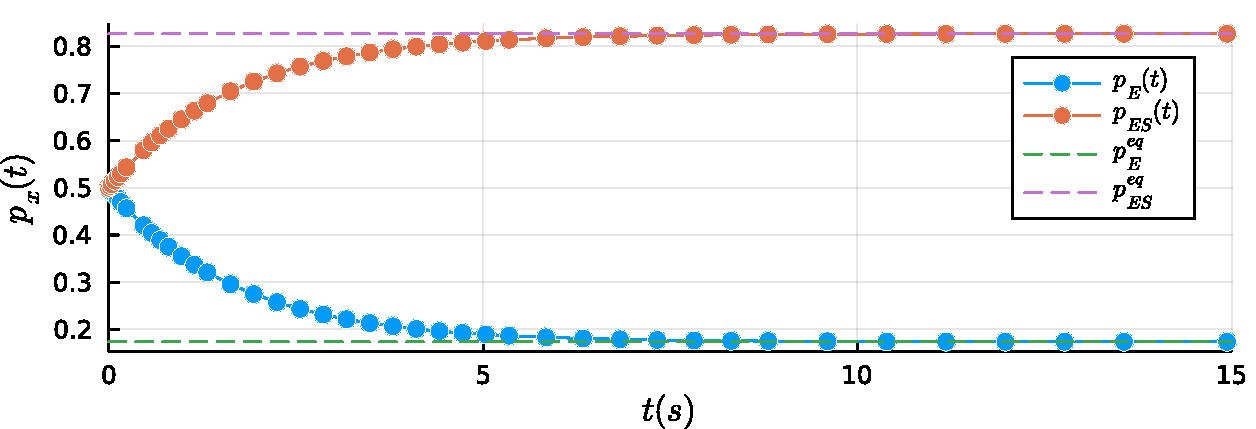
\includegraphics[scale=1.2]{graphics/f1.pdf}
%\end{center}
%\label{fig 2-state-system}
%\caption{\justifying  Time evolution of the probability of the states of the system, $p_E$ and $p_{ES}$, and the probability of the states for the system at in equilibrium, $p_E^{eq}$ and $p_{ES}^{eq}$, with $k_{1} = 0.5$, $k_{-1} = 0.005$, $k_{2} = 0.1$ and $k_{-2} \approx 0.0$.}
%\end{figure}
%
%\begin{figure}
%%\vskip-30pt 
%\begin{center}
%%\includesvg[scale=1.25]{graphics/ST-MM-2.svg}
%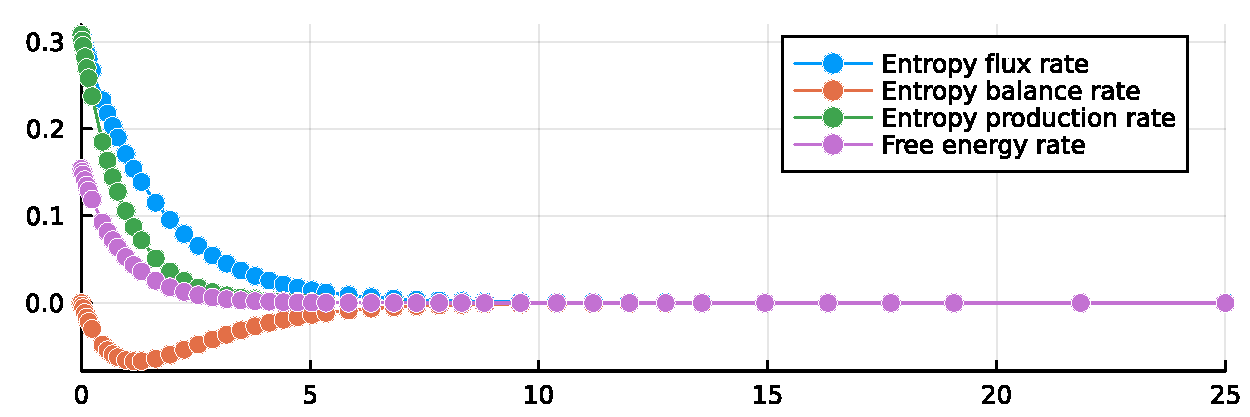
\includegraphics[scale=1.2]{graphics/f2.pdf}
%\end{center}
%\label{fig 2-state-system}
%\caption{\justifying Average entropy flux rate, average entropy production rate, free energy rate and average entropy balance rate.}
%\end{figure}
%
%%Below are shown 5 different trajectories of the system and the thermodynamic observables in each one.
%
\begin{figure}
%\vskip-30pt 
\begin{center}
%\includesvg[scale=1.25]{graphics/ST-MM-2.svg}
%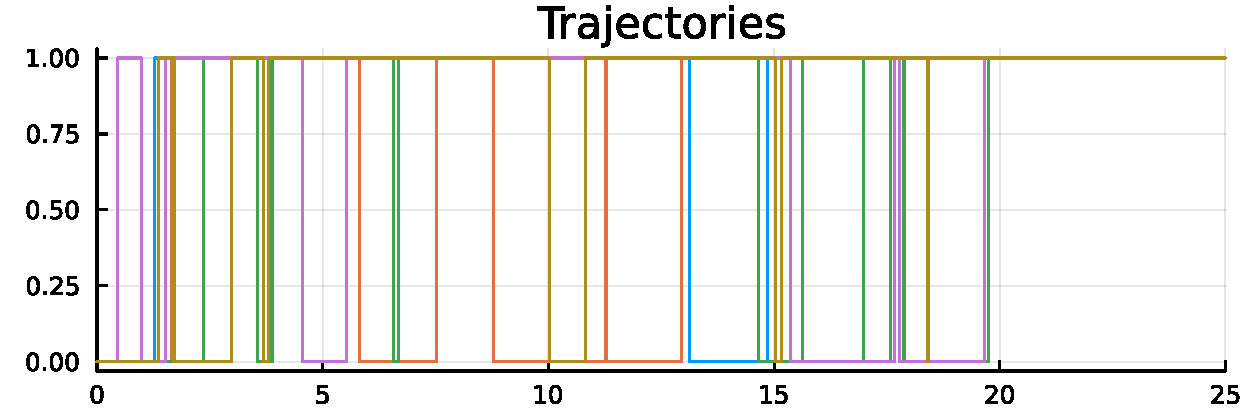
\includegraphics[scale=1.2]{graphics/f6.pdf}
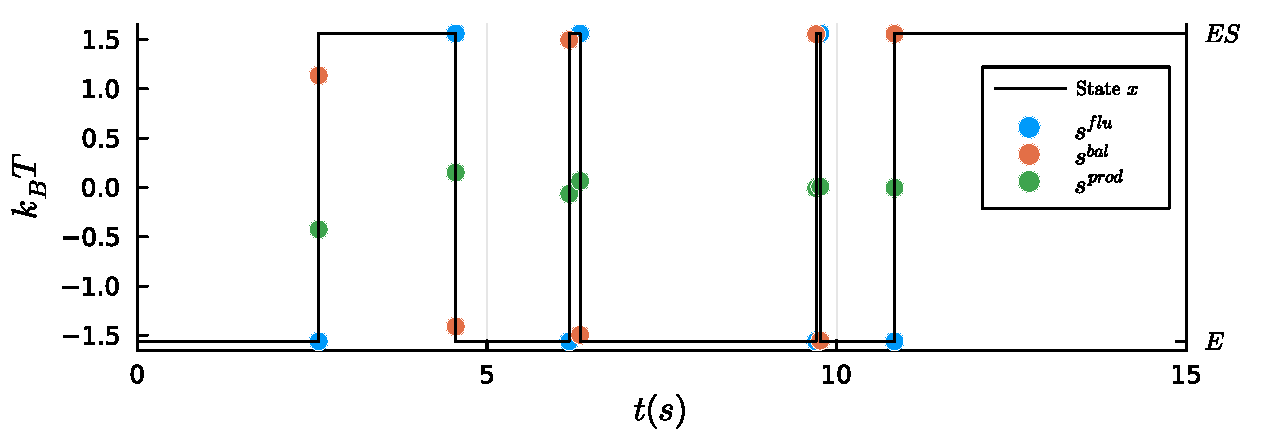
\includegraphics[scale=1.2]{graphics/f8.pdf}
\end{center}
\caption{\justifying Single trajectory of the Markov jump process for the Michaelis-Menten with $k_{1} = 0.5$, $k_{-1} = 0.005$, $k_{2} = 0.1$ and $k_{-2} \approx 0.0$.}\label{fig transition}
\end{figure}


%\begin{figure}
%%\vskip-30pt 
%\begin{center}
%%\includesvg[scale=1.25]{graphics/ST-MM-2.svg}
%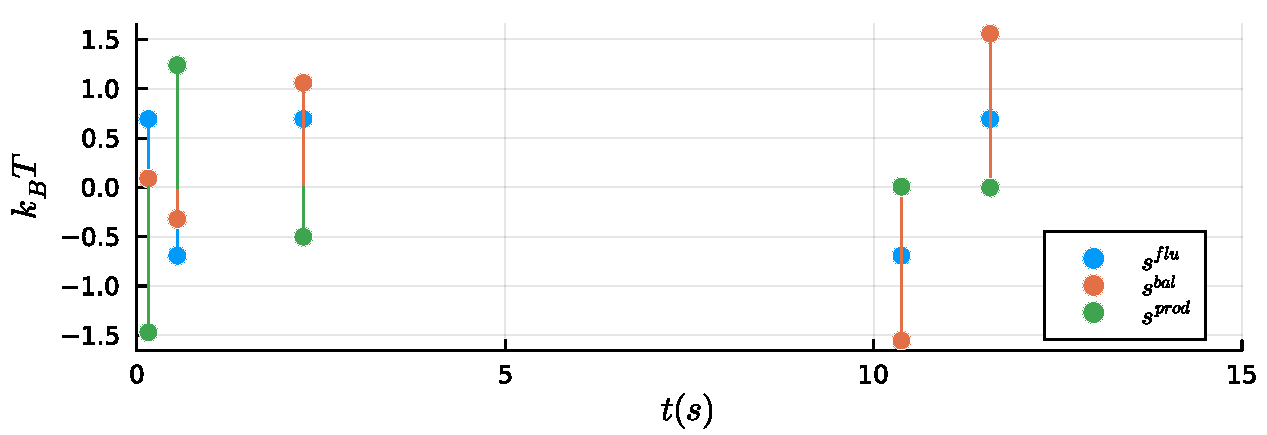
\includegraphics[scale=1.2]{graphics/f7.pdf}
%\end{center}
%\label{fig 2-state-system}
%\caption{Entropy exchange/balance/production for  the trajectory in Fig. \ref{fig transition}.}
%\end{figure}

\begin{figure}
%\vskip-30pt 
\begin{center}
%\includesvg[scale=1.25]{graphics/ST-MM-2.svg}
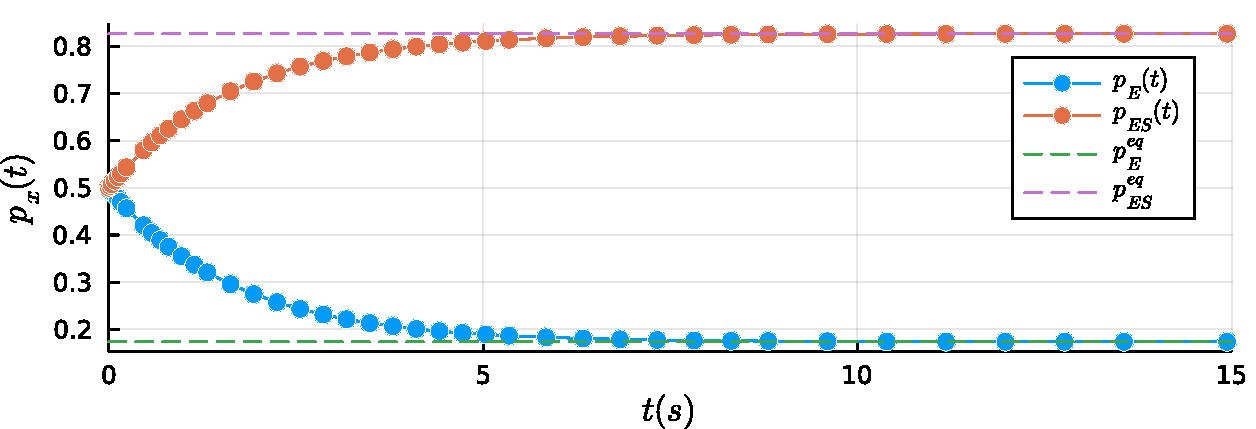
\includegraphics[scale=1.2]{graphics/f1.pdf}
\end{center}
\label{fig 2-state-system}
\caption{\justifying  Time evolution of the probability of the states of the system, $p_E$ and $p_{ES}$, and the probability of the states for the system in equilibrium, $p_E^{eq}$ and $p_{ES}^{eq}$.}
\end{figure}

\begin{figure}
%\vskip-30pt 
\begin{center}
%\includesvg[scale=1.25]{graphics/ST-MM-2.svg}
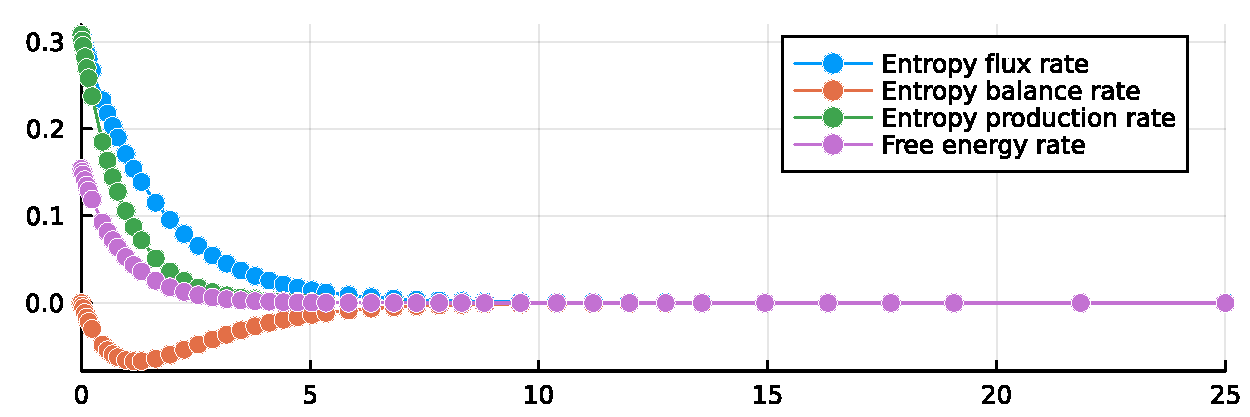
\includegraphics[scale=1.2]{graphics/f2.pdf}
\end{center}
\label{fig 2-state-system}
\caption{\justifying Average entropy flux rate, average entropy production rate, free energy rate and average entropy balance rate.}
\end{figure}

Some conclusions are:
%
\begin{itemize}
\justifying
\item The system relaxes to the equilibrium and, once there, it stabilizes at reservoir properties (e.g. intensive quantities as temperature, chemical potential, etc.);
\item The nonequilibrium free energy of the system is greater than the equilibrium one, thus indicating that work can be exchanged between the system and the reservoir before it gets equilibrated;
\item To sustain the nonequilibrium, work must be applied to the system, which is object of future investigations;
\item The evaluation of the quantities $s^{prod}$, $s^{bal}$, their respective average rates $\dot{S}^{flu}$, $\dot{S}^{prod}$, and $\dot{S}^{bal}$ is only possible because of the numerical solution of \eqref{eq CME}, which is hard to solve for systems with large number of particles. The conventional approach is to use Gillespie algorithm to obtain an ensemble of trajectories;
\item Future explorations are needed to compare the results of the entropies evaluated with the ensemble of trajectories and the numerical integration of \eqref{eq CME}.
\end{itemize}


\end{block}
%
%%The system reaches the steady-state, which for the case of study happens to be also the equilibrium in about 10 seconds:
%%
%%\begin{itemize}
%%\item Both\cite{Qian_2021} the thermodynamic force and flux vanish in the steady-state, which is also an equilibrium.
%%
%%
%%
%%
%%%\item It can be verified that the system obeys {\bf detailed balance}, which connects the math and the physics by recovering the Boltzmann distribution.
%%
%%\item It can be noticed also that all the free energy is used to produce entropy.
%%
%%\item This could be different if one realize work on the system, and it's subject of further research.
%%\end{itemize}
%\end{block}


\end{column}

\separatorcolumn
\end{columns}
 \end{frame}
\end{document}
